\documentclass[12pt]{article}

\usepackage{sbc-template}
\usepackage{graphicx,url}
\usepackage[utf8]{inputenc}
\usepackage[T1]{fontenc}
\usepackage[provide=*,brazilian]{babel}
\usepackage{booktabs}
\usepackage{amsmath}

\graphicspath{{figuras/}}
\sloppy

\title{Perfis de abastecimento de água e esgotamento sanitário dos municípios
  do estado de São Paulo: uma análise de clusterização comparativa entre 2019 e 2024}

\author{Camila Alves Teixeira da Silva\inst{1}, Carolina Numata Pereira\inst{1},
  Thaís de Lima Peixoto\inst{1}}

\address{Escola de Artes, Ciências e Humanidades -- Universidade de São Paulo (USP)\\
  São Paulo -- SP -- Brasil
  \email{camila.atsilva@usp.br, carolinanumata@usp.br, tpeixoto@usp.br}
}

\begin{document}

\maketitle

\begin{resumo}
  O acesso aos serviços de abastecimento de água e de esgotamento sanitário apresenta distribuição
  desigual entre os territórios. Este trabalho tem como objetivo identificar e caracterizar perfis
  desses serviços nos municípios do estado de São Paulo, comparando dois cortes temporais, 2019 e
  2024, e relacionando os perfis ao porte populacional. São utilizados dados do Sistema Nacional de
  Informações sobre Saneamento (SNIS), referentes a 2019, e do Sistema Nacional de Informações em
  Saneamento Básico (SINISA), referentes a 2024. Após a harmonização das bases, foram selecionados
  quatro indicadores comparáveis entre os sistemas: atendimento total de água, perdas na
  distribuição, atendimento total de esgoto e tratamento do esgoto coletado. Após a exclusão de
  valores implausíveis, a amostra principal reúne 597 dos 645 municípios com os quatro indicadores
  nos dois anos. Resultados preliminares com k-means indicam três perfis, que combinam
  níveis de acesso às redes e de tratamento do esgoto e se distribuem de forma graduada segundo o
  porte. A pesquisa adota abordagem quantitativa, de natureza aplicada e
  objetivos exploratórios e descritivos. Serão comparados três algoritmos de clusterização:
  k-means, agrupamento hierárquico de Ward e modelo de mistura gaussiana, com validação por métricas
  internas, concordância entre algoritmos, reamostragem bootstrap e plausibilidade dos perfis.
\end{resumo}

\begin{abstract}
  Access to water supply and sewage services is unevenly distributed across territories. This study
  aims to identify and characterize profiles of these services in the municipalities of the state
  of São Paulo, comparing two time points, 2019 and 2024, and relating the profiles to population
  size. Data from the National Sanitation Information System (SNIS), for 2019, and from the National
  Basic Sanitation Information System (SINISA), for 2024, are used. After harmonizing the databases,
  four indicators comparable between the systems were selected: total water service coverage,
  distribution losses, total sewage collection coverage and treatment of collected sewage. After
  excluding implausible values, the main sample comprises 597 of the 645 municipalities with all four
  indicators in both years. Preliminary k-means results indicate three profiles that combine levels
  of network access and sewage treatment and are distributed in a graded way across population size
  classes. The research adopts a quantitative approach, with
  an applied nature and exploratory and descriptive objectives. Three clustering algorithms will be
  compared: k-means, Ward's hierarchical clustering and Gaussian mixture models, validated through
  internal metrics, agreement between algorithms, bootstrap resampling and plausibility checks.
\end{abstract}

% =====================================================================================
\section{Introdução}

O saneamento básico constitui um dos principais componentes da infraestrutura urbana e desempenha
papel fundamental na promoção da saúde pública, na preservação ambiental e na qualidade de vida da
população. O acesso adequado aos serviços de abastecimento de água e de esgotamento sanitário está
relacionado às condições de vida da população e à capacidade de planejamento e gestão dos
territórios. Apesar da expansão desses serviços observada no Brasil, a disponibilidade e as
condições de atendimento ainda apresentam diferenças entre municípios e regiões, tornando relevante
a análise de sua distribuição territorial.

No estado de São Paulo, essa questão apresenta particularidades decorrentes da grande diversidade
existente entre seus municípios. O estado reúne municípios com diferentes dimensões populacionais,
características territoriais, estruturas econômicas e formas de organização dos serviços públicos.
Dessa maneira, uma análise baseada exclusivamente em indicadores agregados para todo o estado pode
ocultar diferenças existentes entre os municípios. A observação conjunta de diferentes indicadores
permite investigar como essas características se combinam e identificar municípios que apresentam
padrões semelhantes.

A análise de múltiplas variáveis também é relevante porque diferentes dimensões da infraestrutura
podem apresentar comportamentos distintos dentro de um mesmo município. Um município pode, por
exemplo, apresentar elevada cobertura de abastecimento de água e, simultaneamente, baixa proporção
de esgoto tratado ou perdas elevadas na distribuição. Dessa forma, a análise individual de
indicadores pode não ser suficiente para representar a configuração geral dos serviços. A
identificação de perfis permite considerar simultaneamente diferentes características e observar
combinações recorrentes entre os municípios.

Nesse contexto, técnicas de aprendizado de máquina não supervisionado, especialmente os métodos de
clusterização, constituem uma alternativa para identificar grupos de unidades com características
semelhantes, sem que seja necessário estabelecer previamente quais municípios pertencem a cada
grupo. A utilização de diferentes algoritmos é importante para avaliar a consistência dos
agrupamentos, pois métodos distintos podem produzir soluções diferentes em função de seus
pressupostos. Nesta pesquisa, são comparados o k-means, o agrupamento hierárquico de Ward e o modelo
de mistura gaussiana, representando abordagens particional, hierárquica e probabilística.

Outro aspecto central é a comparação entre 2019, com dados do Sistema Nacional de Informações sobre
Saneamento (SNIS), e 2024, com dados do Sistema Nacional de Informações em Saneamento Básico
(SINISA). Como o período envolve a substituição de um sistema de informação pelo outro, a utilização
conjunta das bases exige uma etapa de harmonização que identifique indicadores efetivamente
comparáveis. Essa etapa levou à delimitação do escopo aos serviços de abastecimento de água e
esgotamento sanitário: os indicadores de resíduos sólidos disponíveis nas duas bases apresentaram
diferenças de definição e de população de referência que comprometem a comparação entre os anos
(Seção~\ref{sec:indicadores}).

A literatura demonstra a relevância da análise das desigualdades territoriais em saneamento e o
potencial da clusterização para identificar grupos de municípios semelhantes
\cite{raupp2017,lima2025,lima2022}, conforme discutido na Seção~\ref{sec:relacionados}.

Diante desse contexto, o objetivo deste trabalho é identificar e caracterizar perfis de
abastecimento de água e esgotamento sanitário dos municípios do estado de São Paulo por meio de
técnicas de clusterização, utilizando dados referentes a 2019 e 2024. Busca-se, especificamente:
(i)~identificar agrupamentos de municípios com características semelhantes; (ii)~comparar os
resultados produzidos por diferentes algoritmos; (iii)~investigar diferenças entre os perfis
observados nos dois cortes temporais; e (iv)~verificar como os perfis se distribuem segundo o porte
populacional dos municípios.

% =====================================================================================
\section{Metodologia}

Esta pesquisa adota uma abordagem aplicada, na medida em que busca fornecer subsídios práticos para
o diagnóstico das condições de saneamento nos municípios do estado de São Paulo \cite{gil2017}.
Quanto aos objetivos, o trabalho assume caráter simultaneamente exploratório e descritivo
\cite{mohajan2020}: exploratório no interesse em identificar agrupamentos de municípios com
características semelhantes, e descritivo na caracterização das variáveis que compõem cada perfil e
na comparação entre os dois cortes temporais.

Adota-se uma abordagem quantitativa, cuja sequência compreende a obtenção e organização das bases, a
seleção de variáveis comparáveis entre os anos, a análise exploratória, o pré-processamento, a
aplicação dos algoritmos de clusterização e a validação dos agrupamentos obtidos.

\subsection{Área de estudo e recorte temporal}

A unidade de análise são os 645 municípios do estado de São Paulo. A análise compreende dois cortes
temporais, 2019 e 2024, tratados como observações distintas e não como uma série temporal contínua:
o objetivo não é modelar a trajetória dos indicadores durante o período intermediário, mas comparar
dois recortes específicos. Essa distinção é importante porque o período envolve uma mudança entre
sistemas de informação e metodologias de coleta; assim, diferenças entre os anos devem ser
interpretadas considerando também as características e limitações de cada fonte.

\subsection{Fontes e harmonização dos dados}

Os dados de 2019 provêm do Diagnóstico dos Serviços de Água e Esgotos do SNIS
\cite{snis2019ae}, organizado por prestador de serviço. Para São Paulo, os dados estão distribuídos
em quatro planilhas de indicadores, segundo o tipo de prestador: regional (SABESP), local de direito
público, local de empresa privada e local de direito privado com administração pública, somando 631
linhas e 628 municípios. Em três municípios (Mauá, Salto e Santa Maria da Serra), os serviços de
água e de esgoto são prestados por entidades distintas; suas linhas foram combinadas para que cada
município corresponda a uma única observação. Os dados de 2024 provêm das bases municipais de água e
de esgoto do SINISA, ano de referência 2024 \cite{sinisa2025}; utilizou-se a versão retificada da
base de água (25/05/2026).

A harmonização compreendeu a padronização dos códigos municipais, a identificação dos indicadores
correspondentes e a verificação da cobertura. O SNIS identifica os municípios pelo código do IBGE sem
o dígito verificador (seis dígitos), enquanto o SINISA usa o código completo (sete dígitos); a junção
foi feita removendo o último dígito do código do SINISA. A correspondência entre indicadores seguiu
os glossários oficiais de indicadores dos dois sistemas.

O porte populacional foi obtido da população total residente informada no SINISA 2024 (variável
DFE0001). Os municípios foram classificados em cinco faixas: até 20 mil habitantes (391 municípios),
de 20 a 50 mil (116), de 50 a 100 mil (58), de 100 a 250 mil (46) e acima de 250 mil (34). Uma única
referência populacional foi usada para os dois anos, de modo que mudanças de faixa não se confundam
com mudanças de perfil. O porte não entra na formação dos agrupamentos; ele é usado posteriormente
para caracterizar os perfis.
% PENDENTE: citar referência bibliográfica para as faixas de porte.

\subsubsection{Indicadores selecionados}
\label{sec:indicadores}

Foram selecionados quatro indicadores, dois relacionados ao acesso aos serviços e dois à qualidade e
eficiência de sua prestação (Tabela~\ref{tab:indicadores}). Todos são expressos em percentual.

\begin{table}[ht]
\centering
\caption{Indicadores selecionados e correspondência entre SNIS (2019) e SINISA (2024).}
\label{tab:indicadores}
\small
\begin{tabular}{llll}
\toprule
Variável & Dimensão & 2019 (SNIS) & 2024 (SINISA) \\
\midrule
Água (atendimento total)        & acesso     & IN055 & IAG0001 \\
Esgoto (atendimento total)      & acesso     & IN056 & IES0001 \\
Tratamento do esgoto coletado   & qualidade  & IN016 & IES2004 \\
Perdas na distribuição          & eficiência & IN049 & IAG2013 \\
\bottomrule
\end{tabular}
\end{table}

A variável \emph{água} representa o percentual da população total do município atendida por rede
de abastecimento de água: em 2019, o Índice de Atendimento Total de Água (IN055); em 2024, o
Atendimento da População Total com Rede de Abastecimento de Água (IAG0001).

A variável \emph{esgoto} representa o percentual da população total atendida por rede coletora de
esgoto: em 2019, o Índice de Atendimento Total de Esgoto Referido aos Municípios Atendidos com Água
(IN056); em 2024, o Atendimento da População Total com Rede Coletora de Esgoto (IES0001). Essa
variável refere-se à cobertura da rede coletora, e não ao tratamento.

A variável \emph{tratamento} representa o percentual do esgoto coletado que recebe tratamento: em
2019, o Índice de Tratamento de Esgoto (IN016); em 2024, o indicador Esgoto Tratado Referido ao
Esgoto Coletado (IES2004). Valor zero indica município que coleta esgoto sem tratá-lo.

A variável \emph{perdas} representa o percentual do volume de água disponibilizado para distribuição
que não é contabilizado como consumido: em 2019, o Índice de Perdas na Distribuição (IN049); em
2024, as Perdas Totais de Água na Distribuição (IAG2013). Diferentemente das demais, valores mais
altos indicam pior desempenho. A correspondência é declarada no glossário do SINISA, mas a
composição dos volumes utilizados no cálculo apresenta pequenas diferenças entre os sistemas, o que
torna esta a variável de comparabilidade mais frágil do conjunto.

Indicadores de resíduos sólidos (cobertura da coleta domiciliar e massa coletada per capita) foram
avaliados e excluídos da matriz. Entre SNIS e SINISA, a cobertura da coleta passou de um conceito de
coleta ``regular'' para coleta ``direta ou indireta'', e a massa per capita passou a ser calculada
sobre a população total, e não mais sobre a população atendida. A correlação de Spearman entre os
valores de 2019 e 2024 de um mesmo município foi de apenas 0,35 para a cobertura e 0,18 para a massa,
contra 0,48 a 0,75 nos indicadores de água e esgoto. Além disso, a inclusão de resíduos reduziria a
amostra de 607 para 521 municípios, com perda concentrada nos municípios de até 20 mil habitantes, dos
quais apenas 77,2\% teriam dados completos. Como o porte é uma das dimensões de interesse do
trabalho, essa perda seletiva comprometeria a análise.

\subsection{Análise exploratória dos dados}

Antes da clusterização, os indicadores foram submetidos a uma análise exploratória, com o objetivo
de compreender suas distribuições, identificar valores extremos e inconsistências e investigar as
relações entre as dimensões dos serviços. Foram calculadas medidas de tendência central, dispersão
e assimetria, a proporção de municípios no valor máximo (100\%) e no zero, e as relações entre os
indicadores foram avaliadas pela correlação de Spearman, que mede associações monotônicas sem
pressupor relação linear.

Também foi realizada uma comparação exploratória entre 2019 e 2024 para cada indicador, considerando
apenas os municípios com informação nos dois períodos. Foram examinadas a associação entre os
valores dos dois anos e a proporção de municípios com valores superiores, inferiores ou iguais em
2024. Essa comparação não é interpretada diretamente como evidência de melhora ou piora, dadas as
limitações de comparabilidade entre SNIS e SINISA.

\subsection{Pré-processamento}
\label{sec:preproc}

A análise principal utiliza apenas os municípios com os quatro indicadores disponíveis nos dois anos
(casos completos), sem imputação, evitando a introdução de informações artificiais que possam alterar
a estrutura dos agrupamentos. Os municípios excluídos são descritos quanto ao porte, para avaliar o
efeito da exclusão sobre a representatividade.

Dois problemas identificados na análise exploratória (Seção~\ref{sec:distribuicoes}) receberam
tratamento específico. O primeiro é o tratamento do esgoto de 129,42\% registrado por Vinhedo em
2024, valor impossível para um percentual do esgoto coletado; ele foi limitado a 100\%, valor
coerente com o registrado pelo município em 2019 (99,71\%). O segundo são os onze municípios com
perdas na distribuição de exatamente 0\% em 2019. Esses valores foram tratados como ausentes, pois
são implausíveis em sistemas reais de distribuição e contraditos pelos próprios dados: os mesmos
municípios registram perdas por ligação também nulas em 2019 e perdas entre 5\% e 47\% em 2024.
Com isso, dez municípios deixam a amostra de casos completos (o décimo primeiro já não tinha
informação de perdas em 2024).

Essas escolhas foram apoiadas por uma análise de cenários. Para cada problema, as alternativas
(manter, limitar ou retirar o valor; e, para as perdas, também excluir a variável da matriz) foram
combinadas em nove cenários, clusterizados com k-means em doze configurações de pré-processamento.
Cada cenário foi comparado ao cenário sem tratamento pelo Índice de Rand Ajustado \cite{hubert1985}.
O tratamento de Vinhedo praticamente não alterou os agrupamentos (ARI $\geq 0{,}98$ em todas as
configurações). A retirada das perdas nulas também teve efeito pequeno na maioria das
configurações, mas, com transformação logarítmica e padronização z-score, os dez valores nulos
concentraram-se em um único grupo pequeno, que deixou de existir após sua retirada. A exclusão da
variável de perdas foi o cenário que mais alterou os agrupamentos, indicando que ela carrega
informação própria sobre a eficiência dos serviços; por isso, a variável foi mantida, e a matriz sem
perdas é usada apenas como análise de sensibilidade.

As variáveis são
padronizadas com um único ajuste sobre os dados de 2019 e 2024 empilhados, de modo que os dois
cortes temporais fiquem no mesmo espaço e os perfis permaneçam comparáveis. Como os indicadores
apresentam forte concentração no valor máximo de 100\%, são comparadas alternativas de transformação
e de padronização, avaliando-se o quanto cada escolha altera os agrupamentos.

\subsection{Algoritmos de clusterização e validação}

Serão comparados três algoritmos de agrupamento não supervisionado: k-means \cite{macqueen1967},
como método de particionamento; agrupamento hierárquico de Ward \cite{ward1963}; e modelo de
mistura gaussiana (GMM). Como os rótulos atribuídos pelos algoritmos são arbitrários, a comparação
entre os resultados não é feita pela numeração dos clusters, mas pelas características das variáveis
que compõem cada agrupamento.

A definição do número de clusters combina dois métodos. O primeiro é o Método da Silhueta
\cite{rousseeuw1987}, avaliado em uma grade de valores de $k$ (de 2 a 10). Para cada instância $i$,
o coeficiente de silhueta é
\begin{equation}
  s(i) = \frac{b(i) - a(i)}{\max\{a(i),\, b(i)\}},
\end{equation}
em que $a(i)$ é a distância média de $i$ às demais instâncias do seu cluster e $b(i)$ é a menor
distância média de $i$ às instâncias de outro cluster. O método indica o valor de $k$ que maximiza a
média de $s(i)$ sobre todas as instâncias.

Outro método amplamente utilizado para determinar o número ideal de clusters é o Método do
Cotovelo. Conforme \cite{nainggolan2019}, o método envolve a análise da variação do Erro Quadrático
Total (SSE) com diferentes valores de $k$:
\begin{equation}
  \mathrm{SSE}(k) = \sum_{j=1}^{k} \sum_{x \in C_j} \lVert x - \mu_j \rVert^2,
\end{equation}
em que $C_j$ é o conjunto de instâncias do cluster $j$ e $\mu_j$ é o seu centroide. O SSE diminui à
medida que $k$ aumenta; o número adequado de clusters corresponde ao ponto a partir do qual o
aumento de $k$ deixa de produzir reduções expressivas do SSE, formando um ``cotovelo''. Para evitar
uma identificação apenas visual, o cotovelo é localizado como o ponto da curva de SSE (de $k = 1$ a
$k = 10$, com os dois eixos normalizados) mais distante da reta que liga seus extremos.

Os valores indicados pelos dois métodos são tratados como \emph{candidatos}, avaliados por quatro
critérios: (a)~silhueta média superior a 0,25, limite abaixo do qual não há estrutura substancial
de grupos \cite{kaufman1990}; (b)~estabilidade, medida pelo ARI médio entre a partição obtida com
todos os dados e as partições de 100 reamostragens bootstrap de municípios, que deve ser de pelo
menos 0,85; (c)~menor cluster com pelo menos 5\% das instâncias; e (d)~caráter multivariado: a
partição não pode ser reproduzida pelo agrupamento de uma única variável (ARI inferior a 0,90 entre
a partição e o k-means aplicado a cada indicador isoladamente). O critério~(d) evita adotar como
perfil multivariado uma solução que equivale a classificar os municípios por um só indicador. É
adotado o maior candidato que atende aos quatro critérios, por oferecer mais detalhe quando mais de
um é adequado; os demais candidatos são descartados. As métricas de Calinski-Harabasz
\cite{calinski1974} e Davies-Bouldin \cite{davies1979} complementam a avaliação da coesão e da
separação dos grupos.

A concordância entre as soluções produzidas pelos diferentes algoritmos será
avaliada pelo Índice de Rand Ajustado (ARI) \cite{hubert1985}. Adicionalmente, será empregada uma
rotina de reamostragem bootstrap para verificar a estabilidade dos agrupamentos e uma análise da
plausibilidade dos perfis, considerando os valores originais das variáveis.

\subsection{Correspondência entre agrupamentos e porte}

Para a comparação entre algoritmos e entre os dois cortes temporais, serão consideradas as
características dos centroides ou parâmetros representativos de cada agrupamento, permitindo
verificar quais perfis permanecem presentes ou se modificam entre 2019 e 2024. A comparação temporal
será realizada a partir da composição dos perfis e da distribuição dos municípios nos agrupamentos
de cada ano. Por fim, a distribuição dos perfis será analisada segundo as faixas de porte
populacional.

O processamento é realizado em Python \cite{geron2019}, com as bibliotecas \texttt{pandas},
\texttt{NumPy}, \texttt{scikit-learn}, \texttt{SciPy}, \texttt{matplotlib} e \texttt{seaborn}. O
código, incluindo a rotina de estabilidade por reamostragem, é disponibilizado junto aos
procedimentos computacionais utilizados, de modo a favorecer a replicabilidade da análise.

% =====================================================================================
\section{Trabalhos Relacionados}
\label{sec:relacionados}

A literatura sobre saneamento básico apresenta diferentes abordagens para identificar desigualdades
territoriais e padrões associados à infraestrutura urbana. Para fundamentar a presente pesquisa,
foram selecionados trabalhos que utilizam técnicas de agrupamento, análise estatística e construção
de indicadores para investigar diferenças nas condições de saneamento em distintas escalas
territoriais.

Um dos trabalhos mais diretamente relacionados à abordagem proposta investiga a relação entre
saneamento básico e educação nos municípios brasileiros por meio de técnicas de clusterização. O
estudo utiliza dados do Censo Demográfico de 2010 e aplica o algoritmo k-means para agrupar os
municípios a partir de indicadores relacionados ao saneamento e à educação, identificando três grupos
com diferentes características socioeconômicas. Entre as variáveis consideradas estão o acesso à
água encanada, a coleta de lixo e indicadores associados à escolaridade \cite{lima2025}.

A utilização do município como unidade de análise e de um método de aprendizado não supervisionado
aproxima esse estudo da proposta desenvolvida neste trabalho, e demonstra como a clusterização pode
revelar padrões que não são facilmente observados na análise isolada dos indicadores. Entretanto, o
estudo utiliza somente informações do Censo de 2010 e combina variáveis de saneamento com
indicadores educacionais. A presente pesquisa diferencia-se ao concentrar a formação dos
agrupamentos em indicadores dos serviços de água e esgoto, ao comparar dois recortes temporais com
dados municipais do SNIS e do SINISA e ao considerar diferentes métodos de agrupamento.

Outra perspectiva é apresentada no estudo sobre as condições de saneamento e as desigualdades de cor
ou raça no Brasil urbano. A pesquisa utiliza microdados do Censo Demográfico de 2010 e considera como
desfechos o abastecimento de água, o esgotamento sanitário, a coleta de lixo e uma medida de
saneamento adequado. A análise combina estatísticas descritivas com modelos de regressão logística
múltipla ajustados por características socioeconômicas e demográficas. Os resultados indicam que o
esgotamento sanitário apresentava as condições mais precárias entre os serviços analisados e
evidenciam desigualdades na disponibilidade de infraestrutura sanitária, especialmente para
domicílios com responsáveis indígenas \cite{raupp2017}.

Embora não utilize técnicas de clusterização, esse estudo é relevante por demonstrar que indicadores
de saneamento devem ser analisados de maneira multidimensional, uma vez que diferentes componentes da
infraestrutura podem apresentar níveis de cobertura distintos. Sua unidade de análise, entretanto, é
o domicílio, enquanto a presente pesquisa considera o município. Além disso, o estudo utiliza um único
recorte temporal, enquanto a análise aqui proposta compara 2019 e 2024.

Uma abordagem territorial mais específica é encontrada na construção do \emph{Urban Health Index}
(UHI) para o município de São Paulo. Nesse estudo, foram utilizados dados do Censo Demográfico de 2010
no nível de setor censitário, considerando sete indicadores relacionados ao acesso a esgoto, coleta
regular de resíduos, disponibilidade de banheiros, abastecimento de água, renda, composição
demográfica e alfabetização. Após a padronização, os indicadores foram agregados em uma única medida
e espacializados, possibilitando a identificação de desigualdades intraurbanas \cite{lima2022}. Os
resultados revelaram diferenças expressivas entre os setores censitários, com razão de disparidade
de 2,95 e coeficiente angular de 0,30, e um padrão de desigualdade entre áreas centrais e
periféricas \cite{lima2022}.

Apesar dessa contribuição, o objetivo do UHI é sintetizar diferentes dimensões em um único índice,
enquanto a presente pesquisa busca preservar a natureza multivariada dos indicadores para identificar
grupos de municípios. Além disso, a escala territorial é distinta: o UHI evidencia desigualdades entre
setores censitários dentro do município de São Paulo, e este trabalho considera os 645 municípios do
estado.

Em conjunto, os trabalhos analisados demonstram a relevância de abordagens quantitativas e
multivariadas para a identificação de desigualdades relacionadas ao saneamento, mas diferem quanto
à unidade territorial, às variáveis, às técnicas e ao período analisado. A presente pesquisa busca
avançar nessa direção ao utilizar indicadores municipais de acesso, qualidade e eficiência dos
serviços de água e esgoto para identificar perfis por meio de diferentes técnicas de clusterização,
em dois momentos distintos e considerando, com as devidas ressalvas, a transição entre o SNIS e o
SINISA.

% =====================================================================================
\section{Resultados Preliminares}

Os resultados a seguir referem-se à análise exploratória dos dados municipais de água e esgoto do
SNIS (2019) e do SINISA (2024). A Tabela~\ref{tab:exemplo} exemplifica a estrutura da base
consolidada para cinco municípios.

\begin{table}[ht]
\centering
\caption{Exemplo da estrutura dos dados utilizados (valores em \%).}
\label{tab:exemplo}
\small
\setlength{\tabcolsep}{4pt}
\begin{tabular}{lrrrrrrrr}
\toprule
 & \multicolumn{4}{c}{2019 -- SNIS} & \multicolumn{4}{c}{2024 -- SINISA} \\
\cmidrule(lr){2-5}\cmidrule(lr){6-9}
Município & Água & Esgoto & Trat. & Perdas & Água & Esgoto & Trat. & Perdas \\
\midrule
São Paulo           &  99,30 & 96,30 &  92,20 & 34,38 &  99,98 &  99,26 &  88,89 & 24,46 \\
Campinas            &  98,09 & 94,66 &  89,25 & 20,70 &  99,80 &  96,61 &  94,03 & 17,46 \\
Santos              & 100,00 & 99,93 & 100,00 & 11,94 &  99,33 &  98,46 & 100,00 &  5,35 \\
Sorocaba            &  98,49 & 98,22 &  97,50 & 36,21 &  98,97 &  98,85 &  97,62 & 34,22 \\
Presidente Prudente & 100,00 & 99,61 & 100,00 & 28,90 & 100,00 & 100,00 & 100,00 & 22,38 \\
\bottomrule
\end{tabular}
\end{table}

\subsection{Disponibilidade dos dados}

Dos 645 municípios, 628 têm os quatro indicadores em 2019 e 618 em 2024. Os 17 municípios sem dados
em 2019 não constam em nenhuma planilha de água e esgoto do SNIS daquele ano. Em 2024, a principal
causa de ausência é o atendimento de esgoto, sem valor para 27 municípios, por ausência na base ou
por o indicador não ter sido calculado. No total, 607 municípios (94,1\%) têm os quatro indicadores
nos dois anos. Após a retirada das perdas nulas de 2019 (Seção~\ref{sec:preproc}), a amostra da análise principal
reúne 597 municípios (92,6\%).

Os 48 municípios fora da amostra são menores que os incluídos (mediana de 9,8 mil contra 14,1 mil
habitantes): 36 têm até 20 mil habitantes, e nenhum tem mais de 250 mil. Ainda assim, a proporção de
municípios na amostra é alta em todas as faixas de porte (Tabela~\ref{tab:porte}), de modo que a
exclusão tem efeito limitado sobre a representatividade por porte.

\begin{table}[ht]
\centering
\caption{Municípios por faixa de porte: total, com os quatro indicadores nos dois anos
  (completos) e na amostra final, após a retirada das perdas nulas de 2019.}
\label{tab:porte}
\small
\begin{tabular}{lrrrr}
\toprule
Faixa de porte (habitantes) & Total & Completos & Amostra final & \% na amostra \\
\midrule
Até 20 mil       & 391 & 363 & 355 &  90,8 \\
20 a 50 mil      & 116 & 110 & 108 &  93,1 \\
50 a 100 mil     &  58 &  56 &  56 &  96,6 \\
100 a 250 mil    &  46 &  44 &  44 &  95,7 \\
Acima de 250 mil &  34 &  34 &  34 & 100,0 \\
\midrule
Total            & 645 & 607 & 597 &  92,6 \\
\bottomrule
\end{tabular}
\end{table}

\subsection{Distribuição dos indicadores}
\label{sec:distribuicoes}

A Figura~\ref{fig:distribuicoes} apresenta os histogramas dos quatro indicadores em 2019 e 2024.
As estatísticas desta seção referem-se aos dados originais, antes dos tratamentos descritos na
Seção~\ref{sec:preproc}.

\begin{figure}[ht]
\centering
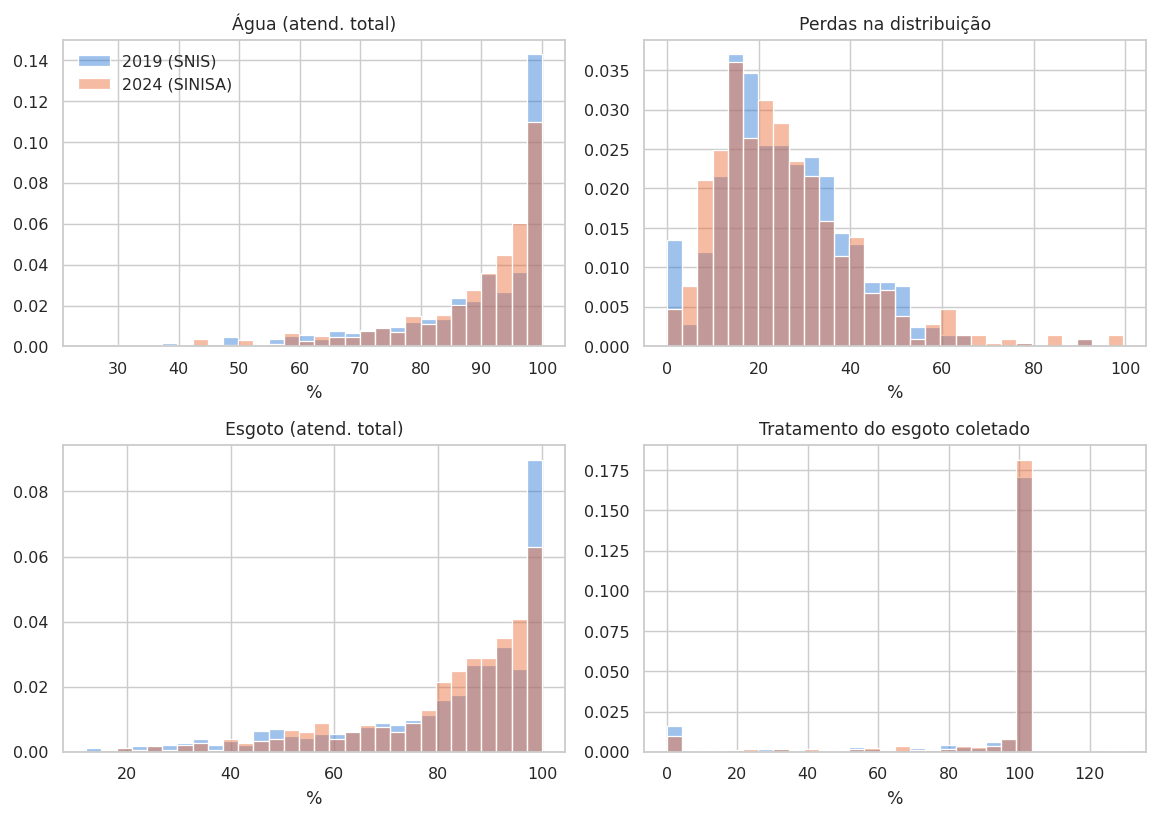
\includegraphics[width=\textwidth]{distribuicoes_2019_2024.png}
\caption{Distribuição dos indicadores em 2019 (SNIS) e 2024 (SINISA).}
\label{fig:distribuicoes}
\end{figure}

Os indicadores de atendimento de água e de esgoto concentram-se nas faixas mais elevadas nos dois
anos. No atendimento de água, a mediana foi de 93,05\% em 2019 e 93,20\% em 2024, e as médias, de
88,34\% e 88,92\%. Há, porém, municípios com percentuais consideravelmente inferiores, com mínimos de
26,82\% em 2019 e 24,77\% em 2024. A proporção de municípios com atendimento de 100\% caiu de
22,93\% para 11,98\%, o que pode refletir tanto mudanças reais quanto a mudança da base populacional
usada no cálculo.

O atendimento de esgoto apresenta maior dispersão. A média passou de 81,90\% para 82,51\%, e as
medianas foram de 88,69\% e 87,88\%. Os mínimos foram de 12,17\% em 2019 e 16,91\% em 2024. A
distância entre os menores valores e a concentração nas faixas superiores evidencia a
heterogeneidade dos municípios paulistas nessa dimensão.

O tratamento do esgoto coletado apresenta a distribuição mais concentrada: a mediana é de 100\% nos
dois anos, e 71,97\% dos municípios em 2019 e 76,97\% em 2024 tratam todo o esgoto coletado. No
extremo oposto, 43 municípios em 2019 e 22 em 2024 coletam esgoto sem tratá-lo (valor zero). Esse
padrão caracteriza um efeito de teto acentuado e uma distribuição praticamente bimodal. Em 2024, o
município de Vinhedo apresenta valor de 129,42\%, fisicamente impossível para um percentual do
esgoto coletado, que foi limitado a 100\% antes da clusterização (Seção~\ref{sec:preproc}).

As perdas na distribuição têm comportamento distinto, com assimetria à direita. A mediana foi de
24,16\% em 2019 e 23,08\% em 2024, e as médias, de 25,52\% e 26,03\%. Enquanto 95\% dos municípios
apresentam perdas de até 50,20\% (2019) e 58,10\% (2024), há valores extremos: sete municípios, seis deles
com até 20 mil habitantes, têm perdas iguais ou superiores a 85\% em 2024, chegando a 99,46\%. Em 2019, onze
municípios registram perdas de exatamente 0\%, valor implausível em sistemas reais de distribuição,
que foi tratado como ausente (Seção~\ref{sec:preproc}). As perdas elevadas de 2024 permanecem na análise, por
serem possíveis, mas devem ser verificadas, pois observações extremas podem influenciar métodos
baseados em distância, como o k-means.

\subsection{Relações entre os indicadores}

A Figura~\ref{fig:correlacao} apresenta as matrizes de correlação de Spearman de 2019 e 2024.

\begin{figure}[ht]
\centering
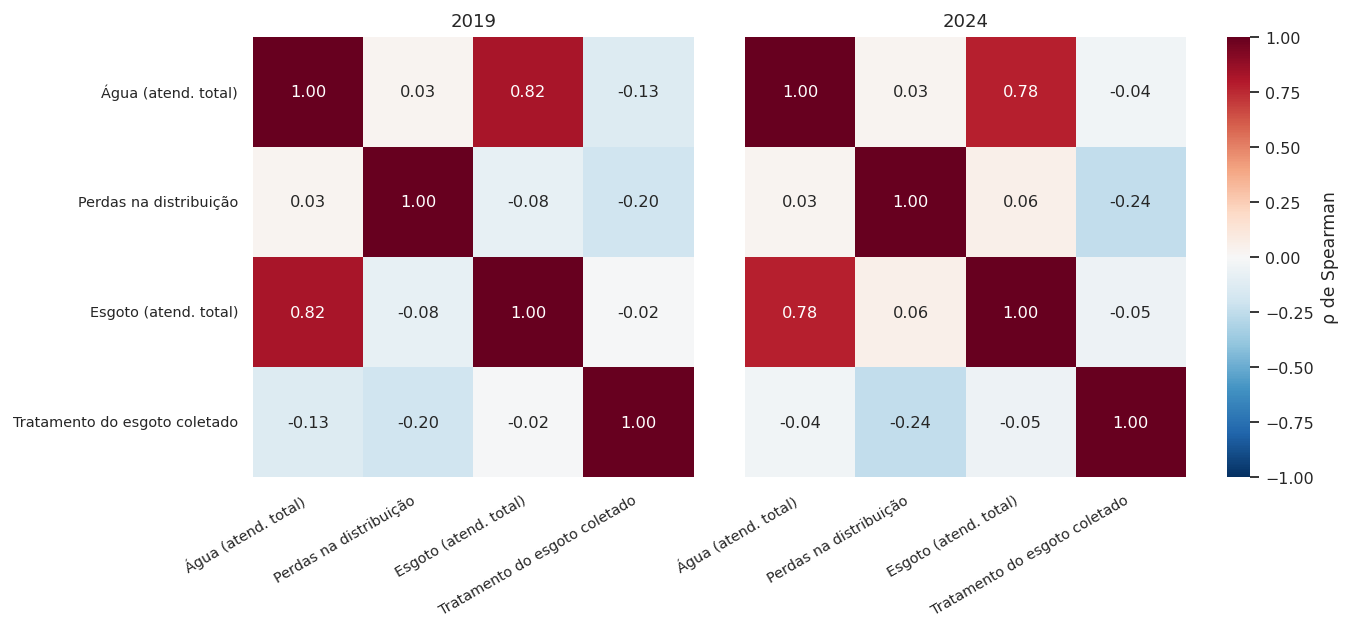
\includegraphics[width=\textwidth]{correlacao_spearman_2019_2024.png}
\caption{Correlação de Spearman entre os indicadores em 2019 e 2024.}
\label{fig:correlacao}
\end{figure}

A associação mais elevada nos dois períodos ocorre entre os atendimentos de água e de esgoto, com
$\rho = 0{,}82$ em 2019 e $\rho = 0{,}78$ em 2024: municípios com atendimento de água relativamente
elevado tendem a apresentar também atendimento de esgoto elevado.

Os indicadores de qualidade e eficiência, por outro lado, são praticamente independentes dos
indicadores de acesso. As correlações das perdas com o atendimento de água e de esgoto ficaram entre
$-0{,}08$ e $0{,}06$ nos dois anos, e as do tratamento com essas variáveis, entre $-0{,}13$ e
$-0{,}02$. A associação mais forte entre os dois indicadores de qualidade e eficiência foi negativa e
fraca, entre perdas e tratamento ($\rho = -0{,}20$ em 2019 e $-0{,}24$ em 2024).

Esses resultados indicam que os quatro indicadores não representam uma única dimensão: o acesso aos
serviços não determina a qualidade de sua prestação. Municípios com atendimento semelhante podem
diferir quanto ao tratamento do esgoto e às perdas, o que reforça o interesse em uma abordagem
multivariada.

\subsection{Comparação entre 2019 e 2024}

A Figura~\ref{fig:dispersao} apresenta os valores de cada município em 2019 (eixo horizontal) e
2024 (eixo vertical), considerando os municípios com informação nos dois anos. A linha tracejada
representa a igualdade entre os períodos. A Tabela~\ref{tab:comparacao} resume a comparação.

\begin{figure}[ht]
\centering
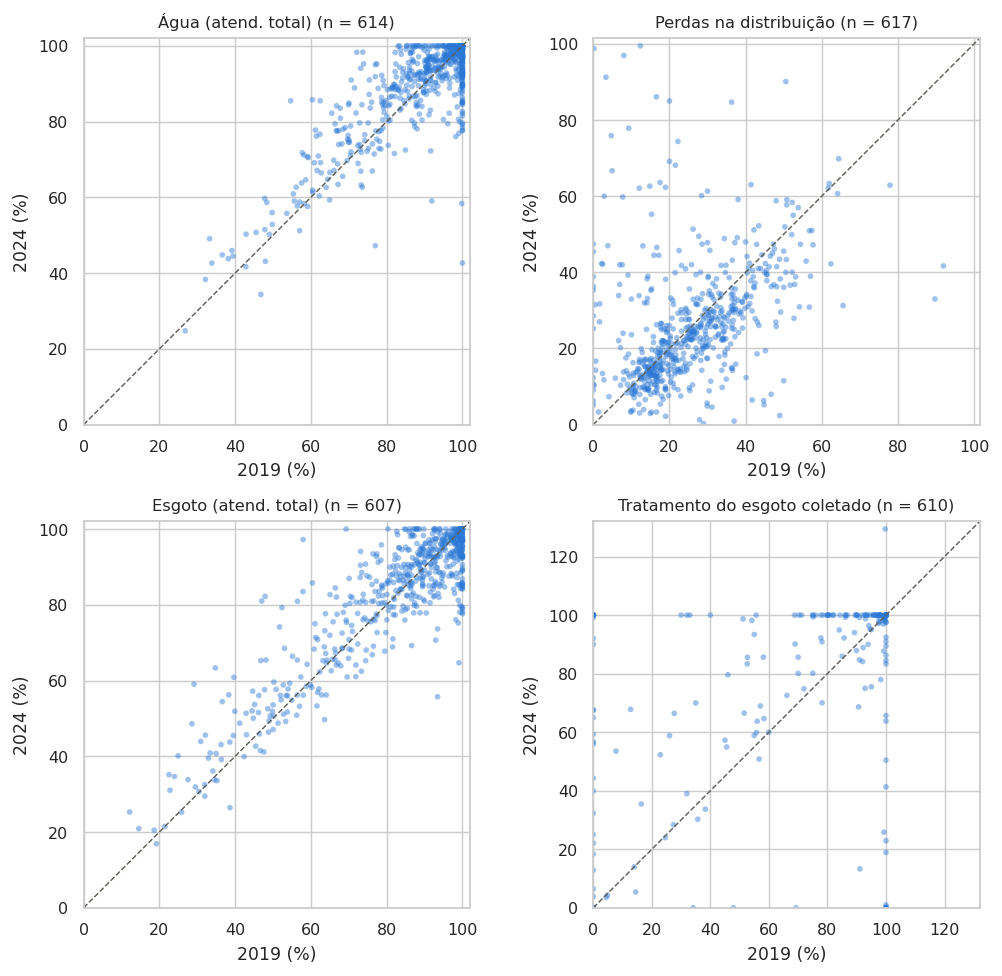
\includegraphics[width=0.85\textwidth]{dispersao_2019_vs_2024.png}
\caption{Valores dos indicadores em 2019 e 2024 para os municípios com dados nos dois anos.}
\label{fig:dispersao}
\end{figure}

\begin{table}[ht]
\centering
\caption{Comparação dos indicadores entre 2019 e 2024 para os municípios com dados nos dois
  períodos. Aumento, redução e igual referem-se ao valor de 2024 em relação ao de 2019.}
\label{tab:comparacao}
\small
\begin{tabular}{lrrrrr}
\toprule
Indicador & N & Aumento (\%) & Redução (\%) & Igual (\%) & $\rho$ \\
\midrule
Água                 & 614 & 51,95 & 42,02 &  6,03 & 0,63 \\
Esgoto               & 607 & 51,89 & 46,95 &  1,15 & 0,75 \\
Tratamento do esgoto & 610 & 19,84 &  9,18 & 70,98 & 0,67 \\
Perdas               & 617 & 37,93 & 61,91 &  0,16 & 0,48 \\
\bottomrule
\end{tabular}
\end{table}

O atendimento de esgoto apresentou a maior associação entre os dois períodos ($\rho = 0{,}75$),
seguido pelo tratamento ($\rho = 0{,}67$) e pelo atendimento de água ($\rho = 0{,}63$), indicando
manutenção da posição relativa dos municípios nessas dimensões. As perdas apresentaram a menor
associação ($\rho = 0{,}48$), resultado coerente com a maior fragilidade da correspondência entre os
dois sistemas para esse indicador.

Nos atendimentos de água e esgoto, a proporção de municípios com aumento foi pouco superior à de
redução (51,95\% contra 42,02\% em água e 51,89\% contra 46,95\% em esgoto). No tratamento, 70,98\%
dos municípios mantiveram o mesmo valor, quase sempre 100\%, e entre os demais predominou o aumento.
Nas perdas, 61,91\% dos municípios apresentaram valores menores em 2024.

Esses resultados não devem ser interpretados diretamente como evidência de melhora ou piora dos
serviços. A comparação envolve a transição do SNIS para o SINISA, com diferenças na estrutura, nas
definições e nos procedimentos de produção das informações; as diferenças observadas podem refletir
tanto alterações efetivas nos municípios quanto mudanças metodológicas.

\subsection{Agrupamentos preliminares com k-means}
\label{sec:agrupamentos}

Como primeiro resultado da etapa de clusterização, o k-means foi aplicado aos 597 municípios nos dois
anos (1.194 municípios-ano), com padronização robusta ajustada sobre 2019 e 2024 em conjunto e
transformação logarítmica com winsorização. Essa configuração de pré-processamento ainda é
provisória. O Método da Silhueta indicou $k = 2$ e o Método do Cotovelo, $k = 3$. A
Tabela~\ref{tab:candidatos} apresenta a avaliação dos dois candidatos.

\begin{table}[ht]
\centering
\caption{Avaliação dos candidatos a número de clusters (k-means, 1.194 municípios-ano).}
\label{tab:candidatos}
\small
\begin{tabular}{lrrrrl}
\toprule
Candidato & Silhueta & Estabilidade & Menor cluster & Uma variável & Resultado \\
 & (a) & (b) & (c) & (d) & \\
\midrule
$k = 2$ (Silhueta) & 0,476 & 0,989 & 19,3\% & 0,965 & descartado (d) \\
$k = 3$ (Cotovelo) & 0,367 & 0,947 & 18,1\% & 0,385 & adotado \\
\bottomrule
\end{tabular}
\end{table}

Os dois candidatos atendem aos critérios de estrutura, estabilidade e tamanho mínimo, mas a solução
com $k = 2$ é quase integralmente reproduzida pelo agrupamento do indicador de tratamento do esgoto
(ARI de 0,965): ela separa os municípios que tratam praticamente todo o esgoto coletado dos demais.
Por isso, foi descartada. A solução com $k = 3$ atende aos quatro critérios e foi adotada. Ela
preserva a separação por tratamento e acrescenta a dimensão de acesso: os municípios que tratam todo
o esgoto coletado dividem-se em dois grupos segundo o nível de acesso às redes
(Figura~\ref{fig:perfis} e Tabela~\ref{tab:perfis}).

\begin{figure}[ht]
\centering
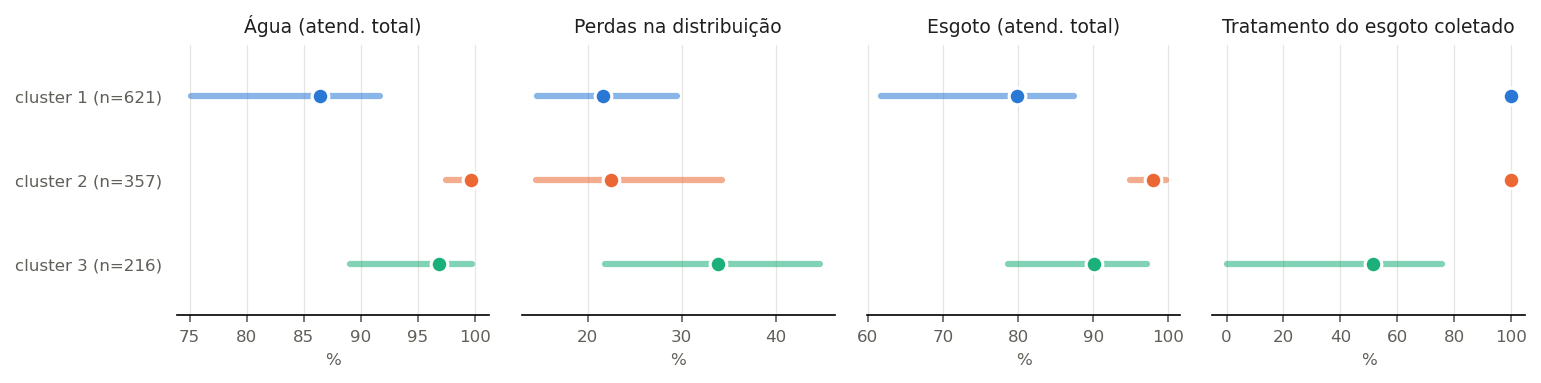
\includegraphics[width=\textwidth]{kmeans_perfis.png}
\caption{Perfis dos três clusters: mediana (ponto) e intervalo interquartil (barra) de cada
  indicador, em unidades originais (1.194 municípios-ano).}
\label{fig:perfis}
\end{figure}

\begin{table}[ht]
\centering
\caption{Perfis dos três clusters: mediana e intervalo interquartil (\%), número de
  municípios por ano e distribuição por faixa de porte (\% dos municípios-ano de cada faixa).}
\label{tab:perfis}
\small
\setlength{\tabcolsep}{4pt}
\begin{tabular}{lrrr}
\toprule
 & Cluster 1 & Cluster 2 & Cluster 3 \\
\midrule
Água          & 86,4 [75,1--91,6] & 99,7 [97,5--100] & 96,8 [89,0--99,7] \\
Esgoto        & 79,8 [61,8--87,5] & 97,9 [94,9--99,7] & 90,0 [78,7--97,1] \\
Tratamento    & 100 [100--100]    & 100 [100--100]    & 51,4 [0,0--75,6] \\
Perdas        & 21,7 [14,7--29,5] & 22,5 [14,5--34,3] & 33,8 [21,8--44,7] \\
Municípios 2019 / 2024 & 306 / 315 & 176 / 181 & 115 / 101 \\
\midrule
Até 20 mil       & 66,5 & 24,2 &  9,3 \\
20 a 50 mil      & 41,7 & 36,1 & 22,2 \\
50 a 100 mil     & 32,1 & 36,6 & 31,2 \\
100 a 250 mil    & 19,3 & 44,3 & 36,4 \\
Acima de 250 mil &  8,8 & 39,7 & 51,5 \\
\bottomrule
\end{tabular}
\end{table}

O cluster~1 reúne municípios que tratam todo o esgoto coletado, mas com acesso intermediário às
redes de água e de esgoto. O cluster~2 combina acesso quase universal e tratamento total. O
cluster~3 apresenta bom acesso, porém tratamento parcial ou ausente e perdas maiores. A distribuição
por porte é graduada: o cluster~1 concentra 66,5\% dos municípios-ano de até 20 mil habitantes e
apenas 8,8\% dos acima de 250 mil, enquanto o cluster~3 segue o padrão inverso (9,3\% e 51,5\%).
Entre 2019 e 2024, 429 dos 597 municípios permaneceram no mesmo cluster; os demais se dividem entre
mudanças em várias direções, como 50 municípios que passaram do cluster~1 para o~2 e 54 que fizeram o
caminho inverso.

A silhueta média da solução adotada (0,367), assim como a do candidato descartado (0,476),
situa-se na faixa que \cite{kaufman1990} associam a estrutura fraca, o que indica que os perfis
devem ser lidos como tendências, e não como grupos nitidamente separados. Esses resultados são preliminares e ainda serão
comparados com o agrupamento hierárquico de Ward e o modelo de mistura gaussiana.

% =====================================================================================
\section{Discussão e conclusão}

A análise exploratória evidencia que os serviços de água e esgoto dos municípios paulistas
apresentam comportamentos distintos conforme a dimensão observada. Os indicadores de acesso
concentram-se em níveis elevados, mas com dispersão e municípios bem abaixo do conjunto principal,
especialmente no esgoto. O tratamento do esgoto coletado é majoritariamente total, mas um grupo de
municípios coleta sem tratar, e as perdas variam amplamente.

A forte associação entre atendimento de água e de esgoto indica que essas dimensões compartilham
parte importante de sua estrutura, enquanto a independência do tratamento e das perdas em relação ao
acesso mostra que a situação dos serviços não pode ser representada por uma única dimensão. Esse
resultado sustenta o uso de técnicas multivariadas de clusterização.

Na comparação entre 2019 e 2024, os indicadores de acesso e de tratamento mantiveram de forma
razoável a posição relativa dos municípios, enquanto as perdas apresentaram menor associação
temporal. Essas diferenças devem ser interpretadas com cautela, uma vez que os dois períodos provêm
de sistemas de informação distintos.

A análise também identificou problemas nos dados. O valor impossível de Vinhedo no tratamento em
2024 foi limitado a 100\%, e as perdas nulas de 2019 foram tratadas como ausentes, o que reduziu a
amostra a 597 municípios. A análise de cenários mostrou que a primeira decisão não altera os
agrupamentos e que a segunda evita, em parte das configurações, a formação de um grupo artificial.
Permanecem como pontos de atenção o efeito de teto no atendimento de água e, sobretudo, no tratamento
do esgoto, e as perdas acima de 85\% em 2024.

Os agrupamentos preliminares com k-means reforçam essa leitura. A solução adotada, com três
perfis, separa os municípios tanto pelo acesso às redes quanto pelo tratamento do esgoto, e o perfil
de acesso intermediário concentra-se nos municípios menores. Já a solução com dois grupos, preferida
pela silhueta, equivale praticamente a uma classificação pelo tratamento do esgoto e foi descartada,
o que mostra a importância de usar critérios adicionais à silhueta na escolha do número de clusters. A estrutura de grupos é,
contudo, fraca, e os perfis devem ser confirmados com outros algoritmos e configurações de
pré-processamento.

As próximas etapas consistem na definição final da transformação e da padronização dos indicadores, seguidas
da aplicação dos métodos k-means, agrupamento hierárquico de Ward e GMM. Os agrupamentos serão
avaliados quanto à qualidade e à estabilidade e caracterizados quanto ao porte populacional. Por
fim, os perfis de 2019 e 2024 serão comparados, considerando as limitações de comparabilidade entre
SNIS e SINISA.

\bibliographystyle{sbc}
\bibliography{referencias}

\end{document}
